% !TeX document-id = {c68f4be8-c497-43e0-82df-e9ebfbea9577}
% !TeX TXS-program:pdflatex = pdflatex -synctex=1 -interaction=nonstopmode --shell-escape %.tex
% новая команда \RNumb для вывода римских цифр
\documentclass[a4paper,12pt]{article}
\usepackage{amssymb}
\usepackage{amsmath}
\usepackage{amsthm} 
\usepackage{caption}
\usepackage{misccorr}
\usepackage[noadjust]{cite}
\usepackage{cmap} 
\usepackage{graphicx}
\usepackage[utf8]{inputenc}
\usepackage[T2A]{fontenc}
\usepackage[english, russian]{babel}
\usepackage{graphics}
\usepackage{graphicx}
\usepackage{textcomp}
\usepackage{verbatim}
\usepackage{makeidx}
\usepackage{geometry}
\usepackage{float}
\usepackage{bm}
\usepackage{esint}
\usepackage{mathtools}
\usepackage{graphicx}
\usepackage{listings}
\usepackage{courier}
\usepackage{multirow}
\usepackage{graphicx}
\usepackage[table]{xcolor}
\usepackage{color}
\usepackage[most]{tcolorbox} 
\usepackage{diagbox}

\lstset{basicstyle=\fontsize{10}{10}\selectfont,breaklines=true}

\newcommand{\specchapter}[1]{\chapter*{#1}\addcontentsline{toc}{chapter}{#1}}
\newcommand{\specsection}[1]{\section*{#1}\addcontentsline{toc}{section}{#1}}
\newcommand{\specsubsection}[1]{\subsection*{#1}\addcontentsline{toc}{subsection}{#1}}
\newcommand{\RNumb}[1]{\uppercase\expandafter{\romannumeral #1\relax}}
\newcommand{\jj}{\righthyphenmin=20 \justifying}


% геометрия
\geometry{pdftex, left = 2cm, right = 2cm, top = 2.5cm, bottom = 2.5cm}

\setcounter{tocdepth}{4} % фикс переноса 
\righthyphenmin = 2
\tolerance = 2048

\begin{document}
	\thispagestyle{empty}
	
	\noindent \begin{minipage}{0.15\textwidth}
		
\includegraphics[width=\linewidth]{b_logo}
	\end{minipage}
	\noindent\begin{minipage}{0.9\textwidth}\centering
		\textbf{Министерство науки и высшего образования Российской Федерации}\\
		\textbf{Федеральное государственное бюджетное образовательное учреждение высшего образования}\\
		\textbf{«Московский государственный технический университет имени Н.Э.~Баумана}\\
		\textbf{(национальный исследовательский университет)»}\\
		\textbf{(МГТУ им. Н.Э.~Баумана)}
	\end{minipage}
	
	\noindent\rule{18cm}{3pt}
	\newline\newline
	\noindent ФАКУЛЬТЕТ $\underline{\text{«Информатика и системы управления»}}$ \newline\newline
	\noindent КАФЕДРА $\underline{\text{«Компьютерные системы и сети»}}$\newline\newline
	\noindent НАПРАВЛЕНИЕ ПОДГОТОВКИ $\underline{\text{«09.03.04 Программная инженерия»}}$\newline\newline\newline\newline\newline
	
	
	\begin{center}
		\noindent\begin{minipage}{1.3\textwidth}\centering
			\Large\textbf{  Рубежный контроль по  }\newline
			\Large\textbf{ дисциплине <<Архитектура ЭВМ>>}\newline\newline\newline
			\textbf{Организация операций сложения, }\newline
			\textbf{вычитания, умножения и деления}\newline
			\textbf{над числами с плавающей запятой}\newline\newline\newline\newline
		\end{minipage}
	\end{center}
	
	\begin{center}
		\begin{tabular}{ccccc}
			Студент: & $\underline{\text{ИУ7-53Б}}$ & $\underline{\text{~~~~~~~~~~~}}$ & $\underline{\text{23.12.2020}}$ & $\underline{\text{А. В. Романов}}$ \\
			& \footnotesize группа & \footnotesize подпись & \footnotesize дата  & \footnotesize (И. О. Фамилия) \\
			&  &  &  & \\
			Преподаватель: & \textbf{} & $\underline{\text{~~~~~~~~~~~}}$ & $\underline{\text{~~~~~~~~~~~~}}$ & $\underline{\text{А. Ю. Попов}}$ \\
			&  & \footnotesize подпись & \footnotesize дата  & \footnotesize (И. О. Фамилия) \\
		\end{tabular}
	\end{center}
	
	
	\begin{center}
		\vfill
		Москва~---~\the\year
		~г.
	\end{center}
	\clearpage

	На рисунке показано представление чисел с плавающей запятой. Мантисса M числа представляется в нормализованном виде, то есть старший разряд не сохраняется.
	
	\begin{center}
		\noindent 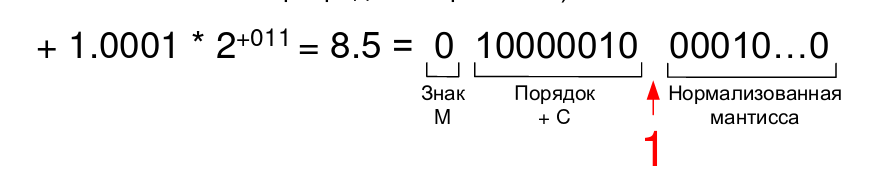
\includegraphics[scale=0.4]{2.png}\newline
	\end{center}

	Так же существуют \textbf{специальные числовые значения}, такие как $-\infty$ , $+\infty$ и другие (представлены на рисунке). Нужны, например, чтобы обрабатывать исключительные операции, такие как деление 0 и прочие.
	
	\begin{center}
		\noindent 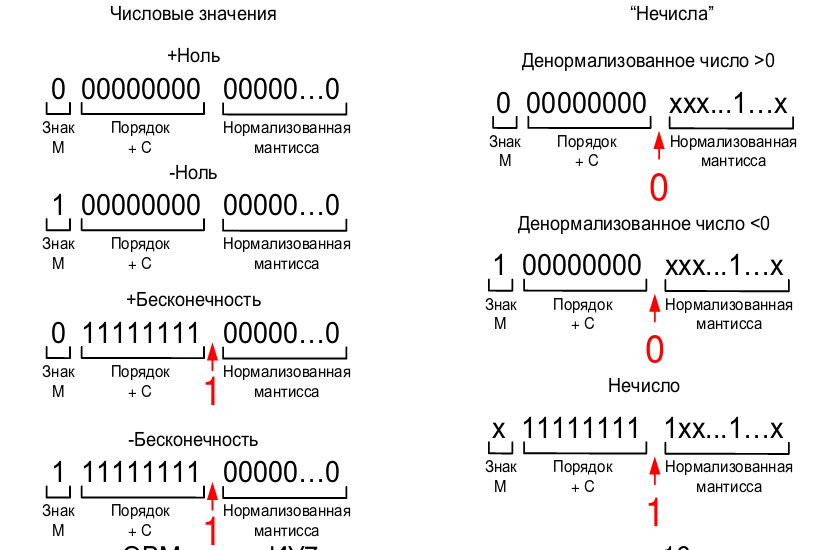
\includegraphics[scale=0.6]{3.png}\newline
	\end{center}


	Операции над числами с плавающей запятой представлены в три этапа:
	
	\begin{enumerate}
		\item \textbf{Подготовительный этап (загружаем число в АЛУ)}
		\begin{itemize}
			\item упакованное число разделяется на группы: мантисса, порядок и знак.
			\item далее происходит проверка на специальное числовое значение.
		\end{itemize}
		\item \textbf{Выполнение самой операции.}
		\begin{itemize}
			\item приведение порядков;
			\item определение знака результата;
			\item определение мантиссы результата;
			\item определение порядка результата;
			\item проверка на: переполнение, потери значимости мантиссы и порядка, неточности и деления на 0.
		\end{itemize}
		\item \textbf{Заключительный этап (выгружаем из АЛУ)}
		\begin{itemize}
			\item проверка на специальное числовое значение;
			\item нормализация результата;
			\item проверка на: переполнение, потери значимости мантиссы и порядка, неточности;
			\item упаковка полученной мантиссы, порядка и знака.
		\end{itemize}
	\end{enumerate}

	\textbf{Организация операций \textbf{сложения и вычитания}}:
	
	\begin{enumerate}
		\item Подготовительный этап (см. выше).
		\item Определение меньше из двух порядков и выравнивание порядков. Эта операция может привести к потери значимости (можем выйти за 000..., и число будет равно 0). Происходит если очень большая разница в порядках.
		\item Проверка на потерю значимости одного операнда.
		\item Определение результирующего порядка как максимума.
		\item Сложение мантисс и определение знака результата.
		\item Проверка на переполнение мантиссы.
		\item Проверка на переполнение порядка.
		\item Заключительный этап (см. выше).
	\end{enumerate}
	
	\textbf{Организация операций \textbf{умножения}}:

	\begin{enumerate}
		\item Подготовительный этап.
		\item Происходит проверка что первая мантисса или вторая равна нулю. Если условие истинно, то .
		\item Определяют порядок результата: порядок первого числа + порядок второго числа - смещение.
		\item Проверка на переполнение порядка.
		\item Определяют мантиссу результата: мантисса первого числа * мантисса второго числа.
		\item Определяют знак результата.
		\item Заключительный этап.
	\end{enumerate}

	\textbf{Организация операций \textbf{деления}}:

	\begin{enumerate}
		\item Подготовительный этап.
		\item Происходит проверка что первая мантисса или вторая равна нулю. Если происходит деление на ноль, то сразу определяется $+-\infty$ (либо ошибка деления на 0).
		\item Определяют порядок результата: порядок первого числа - порядок второго числа + смещение.
		\item Проверка на переполнение порядка.
		\item Определяют мантиссу результата: мантисса первого числа * (1 / мантисса второго числа). Обратная величина вычисляется разложением в ряд.
		\item Определяют знак результата.
		\item Заключительный этап.
	\end{enumerate}
	
		""\newline
	При делении чисел с  плавающей запятой не делятся (как в случае целочисленного деления), а умножаются на обратное. Благодаря этому выигрывается время. 

\end{document}